\subsection{Payload}
The pneumatic parellel gripper, manual quick-change system and robotic camera constitutes a weight of 2.0 kg.
This is the payload on the tool flange center (\hyperref[acro:TFC]{TFC}). The sheet metal parts does not weigh much,
so are ignored in the calculations.


\begin{figure}[h]
    \centering
    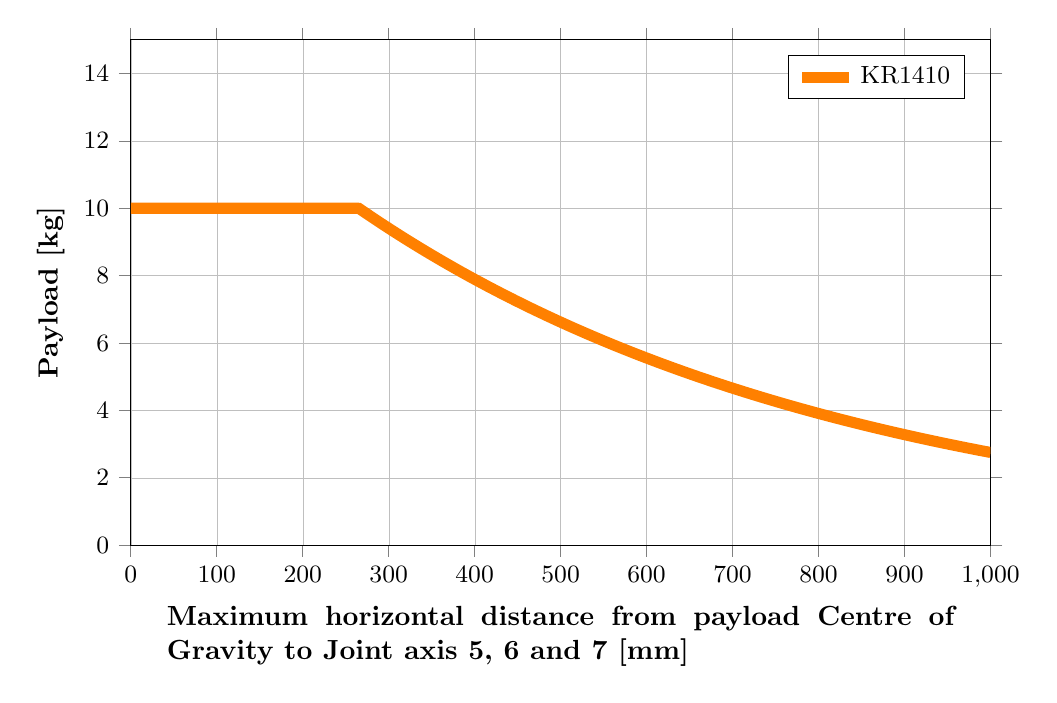
\begin{tikzpicture}
        \begin{axis}[
            width=12.5cm,
            height=8cm,
            grid=both,
            grid style={line width=.1pt, draw=gray!30},
            major grid style={line width=.1pt,draw=gray!50},
            xlabel={\parbox{10cm}{Maximum horizontal distance from payload Centre of Gravity to Joint axis 5, 6 and 7 [mm]}},
            ylabel={\textbf{Payload [kg]}},
            xmin=0, xmax=1000,
            ymin=0, ymax=15,
            legend pos=north east,
            legend style={font=\small},
            ylabel near ticks,
            xlabel near ticks,
            tick align=outside,
            tick label style={font=\small},
            label style={font=\bfseries},
        ]
    
        % KR1410 (orange)
        \addplot [
            color=orange,
            line width=4pt,
            % ultra thick,
            domain=0:1000,
            samples=1000,
        ]
        {x <= 265 ? 10 : 10*exp(-0.001756*(x-265))};
        \addlegendentry{KR1410}
        \end{axis}
    \end{tikzpicture}
    
    \caption{Payload diagram for KR1410 manipulator}
    \label{fig:kr1410-payload-diagram}
\end{figure}


The permissible payload is constrained due to the static torque limit of the wrist joints. The payload is
reduced according to the proximity of the payload's centre of gravity in relation to joint axis 5, 6 and 7. \cite[page 35]{kassow-manual} Figure \ref{fig:kr1410-payload-diagram}
illustrates the allowable payload as a function of distance.

\subsection{Stopping Distance}
According to \cite[page 35]{kassow-manual}, the time and distance it takes to stop the robot, for instance with an emergency stop or protective stop, depends on the load, speed
and configuration of the robot.

\begin{table}[h]
    \centering
    \renewcommand{\arraystretch}{1.2} % Adjusts row height
    \setlength{\tabcolsep}{4pt} % Adjusts column spacing
    \begin{tabular}{|c|c|*{8}{c|}}
        \hline
        \textbf{Load} & \textbf{Direction} & 
        \multicolumn{8}{c|}{\textbf{Distance from Joint axis 1 or 2 to Load center of gravity or TFC whichever is larger}} \\
        \cline{3-10}
        \textbf{[kg]} & \textbf{[kg]} & 800-950 & 700-800 & 600-700 & 500-600 & 400-500 & 300-400 & 0-300 \\
        \hline
        \multirow{4}{*}{0-4}  & 0-40  & 895  & 1026 & 1304 & 1663 & 2131 & 2724 & 3437 \\
                              & 40-80 & 1433 & 1578 & 1745 & 2132 & 2522 & 3131 & 3724 \\
                              & 80-120 & 1378 & 1549 & 1720 & 2115 & 2643 & 3165 & 4045 \\
                              & 120-160 & 1861 & 2040 & 2371 & 2773 & 3259 & 3824 & 4342 \\
        \hline
    \end{tabular}
    \caption{Braking accelerations for KR1410}
    \label{tab:braking_accelerations}
\end{table}
